\documentclass[8pt,aspectratio = 169]{beamer}

\usetheme[sectionpage=none, subsectionpage=progressbar]{metropolis}
\setbeamertemplate{footline}[frame number] % Mantém apenas o número do slide
\setbeamertemplate{navigation symbols}{} % Remove símbolos de navegação padrão
\hypersetup{pdfpagemode=FullScreen}
\hypersetup{pdfpagelayout=SinglePage}

%-------------------------------------------------------
% INCLUDE PACKAGES
%-------------------------------------------------------

\usepackage[utf8]{inputenc}
\usepackage[english,brazil]{babel}
\usepackage[T1]{fontenc}
\usepackage{helvet}
\usepackage[num]{abntex2cite}
\citebrackets[]
\usepackage{pgfplots}
\usepackage{amsmath}
\usepackage{amsfonts}
\usepackage{amssymb}
\usepackage{pdflscape}
\usepackage{afterpage}
\usepackage{capt-of}
\usepackage{booktabs}
\usepackage{array}
\usepackage{multirow}
\usepackage{longtable}
\usepackage{siunitx} 
\newcolumntype{T}[1]{S[table-format=#1]}
\newcommand\mc[1]{\multicolumn{1}{c}{#1}}
\usepackage{graphicx}
\usepackage{caption}
\usepackage{tikz} 
\usetikzlibrary{decorations.pathreplacing} % Biblioteca TikZ para as chaves ({})
\usepackage{cancel}
\usepackage{xcolor}

% Configuração das molduras ao redor das figuras e tabelas da seção 7.3
\setlength{\fboxsep}{4pt}
\setlength{\fboxrule}{0.8pt}

%-------------------------------------------------------
% DEFINING AND REDEFINING COMMANDS
%-------------------------------------------------------
\newcommand{\chref}[2]{
  \href{#1}{{\usebeamercolor[bg]{Feather}#2}}
}

%-------------------------------------------------------
% INFORMATION IN THE TITLE PAGE
%-------------------------------------------------------
\title[]{ \textbf{Soluções das EDOs por Séries.} }

\subtitle[]{ Funções especiais }

\author[L. Silva]{ \normalsize Autores: Luiz Felipe Souza de Lima Silva }

\institute[]{
  \small
  Universidade Federal do Pará (UFPA) \\
  Campus Universitário de Tucuruí \\
  Faculdade de Engenharia Elétrica \\
}

\date{2026}

%-------------------------------------------------------
% THE BODY OF THE PRESENTATION
%-------------------------------------------------------

\begin{document}

\begin{frame}[plain,noframenumbering] 
  \titlepage 
\end{frame}

\begin{frame}{Sumário de apresentação}
  \tableofcontents
\end{frame}

%-------------------------------------------------------
\section{Introdução}

\section{Resoluções}

%=====================================================================================
\subsection{Questão 1}

\begin{frame}{Questão 1 - Enunciado}

\begin{figure}[h]
    \centering
    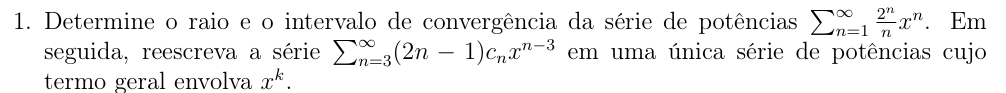
\includegraphics[width=0.8\textwidth]{q1.png}
\end{figure}

\setbeamercolor{block title}{bg=structure.fg, fg=white}
\setbeamercolor{block body}{bg=structure.fg!10, fg=black}
  
  \begin{block}{Conceito chave:}
    Define-se o intervalo de convergência aplicando a razão de teste no coeficiente $c_n$:
    \[
    \text{Seja}: \quad \sum_{n=0}^{\infty} c_n (x - a)^n
    \]
    \[
    \text{Aplicamos o teste da razão aos coeficientes } c_n: \quad L = \lim_{n \to \infty} \left| \frac{c_{n+1}}{c_n} \right|
    \]
    O raio será o inverso de $L$ e o intervalo de convergência por definição é $|x| < R = \frac{1}{2}$.
  \end{block}

\end{frame}


\begin{frame}[allowframebreaks]{Questão 1 - Resolução}

    Temos a série:
    \[ 
    \sum_{n=1}^{\infty} \frac{2^n}{n} x^n \qquad \implies \qquad c_n = \frac{2^n}{n} 
    \]

    Aplicando o teste da razão:
    \[ 
    L =  \lim_{n \to \infty} \left| \frac{c_{n+1} (x-0)^{n+1}}{c_n (x-0)^n} \right| = \lim_{n \to \infty} \left| \frac{\frac{2^{n+1}}{n+1}}{\frac{2^n}{n}} \right| 
    \]

    Portanto:
    \[ 
    L = |x| \cdot \lim_{n \to \infty} \left| \frac{2^{n+1}}{n+1} \cdot \frac{n}{2^n} \right| = |x| \cdot \lim_{n \to \infty} \left| \frac{2 \cdot n}{n+1} \right| 
    \]

    \[ 
    \therefore L = |x| \cdot \lim_{n \to \infty} \left| \frac{n(2)}{n(1 + \frac{1}{n})} \right| = |x| \cdot \lim_{n \to \infty} \left| \frac{2}{1} \right| = 2|x| 
    \]

    $\therefore$ Raio de convergência $R = \frac{1}{2}$.

    \framebreak 

    Intervalo de convergência ($2|x| < 1$):
    \[ 
    |x| < \frac{1}{2} \implies -\frac{1}{2} < x < \frac{1}{2} 
    \]
    
    A série converge nesse intervalo.

    \vspace{0.5cm}
    \begin{center}
    \begin{tikzpicture}
        % Reta real
        \draw[<-] (-3,0) -- (3,0);
        \node at (-3.2, 0) {$R$};
        
        % Linha ondulada (intervalo de convergência)
        \draw[thick, decorate, decoration={snake, amplitude=0.5mm, segment length=3mm}] (-2,0) -- (2,0);
        
        % Pontos abertos
        \draw[fill=white, thick] (-2,0) circle (0.1) node[below=0.2cm] {$-\frac{1}{2}$};
        \draw[fill=white, thick] (2,0) circle (0.1) node[below=0.2cm] {$\frac{1}{2}$};
    \end{tikzpicture}
    \end{center}
    \vspace{0.5cm}

    \framebreak 

    Reduzindo a segunda expressão do problema: 
    \[
    \sum_{n=3}^{\infty} (2n - 1)c_n x^{n-3}
    \]
    
    Fazendo a mudança de índice $k = n - 3 \Rightarrow n = k + 3$:
    \[
    \text{Portanto:} \quad
    \sum_{k=0}^{\infty} [2(k+3) - 1] c_{k+3} x^k = \sum_{k=0}^{\infty} (2k + 5) c_{k+3} x^k
    \]

\end{frame}

%=====================================================================================
\subsection{Questão 2}

\begin{frame}{Questão 2 - Enunciado}

\begin{figure}[h]
    \centering
    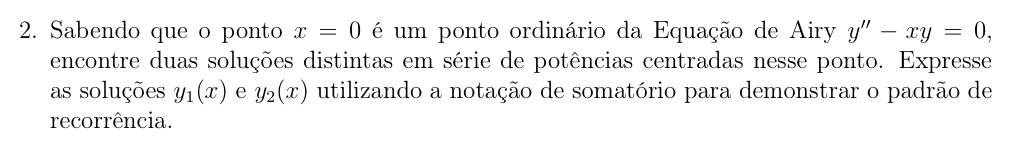
\includegraphics[width=0.8\textwidth]{q2.png}
\end{figure}

\setbeamercolor{block title}{bg=structure.fg, fg=white}
\setbeamercolor{block body}{bg=structure.fg!10, fg=black}

 \begin{block}{Conceito chave:}
    Devido o ponto $x=0$ ser um ponto ordinário (regular), podemos admitir a seguinte hipótese de solução em séries de potências:
    \[ y(x) = \sum_{n=0}^{\infty} C_n x^n \]
 \end{block}
    
\end{frame}

\begin{frame}[allowframebreaks]{Questão 2 - Resolução}
    
    Derivando a série proposta:
    \[ 
    y(x) = \sum_{n=0}^{\infty} C_n x^n \quad ; \quad 
    y'(x) = \sum_{n=1}^{\infty} C_n n x^{n-1} \quad ; \quad 
    y''(x) = \sum_{n=2}^{\infty} C_n n(n-1) x^{n-2} 
    \]

    Substituindo na EDO $y'' - xy = 0$:
    \begin{align*}
        \sum_{n=2}^{\infty} C_n n(n-1) x^{n-2} - x \sum_{n=0}^{\infty} C_n x^n &= 0 \\[1ex]
        \therefore \quad \sum_{n=2}^{\infty} C_n n(n-1) x^{n-2} - \sum_{n=0}^{\infty} C_n x^{n+1} &= 0 
    \end{align*}

    Expandindo os primeiros termos da primeira série para igualar as potências:
    \begin{align*}
        [C_2(2)(1) + C_3(3)(2)x + \dots] - [C_0 x + C_1 x^2 + C_2 x^3 + \dots] &= 0 \\[1ex]
        2C_2 + \sum_{n=3}^{\infty} C_n n(n-1) x^{n-2} - \sum_{n=0}^{\infty} C_n x^{n+1} &= 0 
    \end{align*}

    \framebreak 

    Logo, isolando o termo constante:
    \[ 2C_2 = 0 \implies \boxed{C_2 = 0} \]
    
    Realizando a mudança de variáveis nos índices das somas restantes:
    \[ \sum_{n=3}^{\infty} C_n n(n-1) x^{n-2} - \sum_{n=0}^{\infty} C_n x^{n+1} = 0 \]

    \begin{center}
        \begin{tabular}{cc}
            $n=3$ & $n=0$ \\
            $K = n - 2 \rightarrow n = K + 2$ & $K = n + 1 \rightarrow n = K - 1$
        \end{tabular}
    \end{center}

    Substituindo os índices:
    \[ \sum_{K=1}^{\infty} C_{K+2} (K+2)(K+1) x^K - \sum_{K=1}^{\infty} C_{K-1} x^K = 0  \]

    Agrupando em uma única série:
    \[ \sum_{K=1}^{\infty} x^K [ C_{K+2} (K+2)(K+1) - C_{K-1} ] = 0 \]

    \framebreak 

    Para que a igualdade seja verdadeira para todo $x$, os coeficientes devem ser nulos:
    \[ C_{K+2} (K+2)(K+1) - C_{K-1} = 0 \]

    Como a série inicia em $K=1$, iteramos para encontrar os coeficientes:

    \vspace{0.3cm}
    \noindent P/ $K=1$: \quad $C_3 (3)(2) - C_0 = 0 \implies C_3 = \frac{C_0}{6} = \frac{C_0}{3!}$ 

    \noindent P/ $K=2$: \quad $C_4 (4)(3) - C_1 = 0 \implies C_4 = \frac{C_1}{4 \cdot 3}$ 

    \noindent P/ $K=3$: \quad $C_5 (5)(4) - C_2 = 0 \implies C_5 = 0$ 

    \noindent P/ $K=4$: \quad $C_6 (6)(5) - C_3 = 0 \implies C_6 = \frac{C_3}{6 \cdot 5} = \frac{C_0}{3 \cdot 2 \cdot 6 \cdot 5}$ 

    \noindent P/ $K=5$: \quad $C_7 (7)(6) - C_4 = 0 \implies C_7 = \frac{C_1}{4 \cdot 3 \cdot 7 \cdot 6}$ 

    \noindent P/ $K=6$: \quad $C_8 (8)(7) - C_5 = 0 \implies C_8 = 0$ 

    \framebreak 

    Substituindo os coeficientes encontrados na série original:
    \[ y(x) = \sum_{n=0}^{\infty} C_n x^n = C_0 + C_1 x + C_2 x^2 + C_3 x^3 + \dots \]

    \begin{align*}
        y(x) = & C_0 + C_1 x + \cancel{C_2 x^2}^0 + \frac{C_0}{3!} x^3 + \frac{C_1}{4 \cdot 3} x^4 + \cancel{C_5 x^5}^0 \\
        & + \frac{C_0}{3 \cdot 2 \cdot 6 \cdot 5} x^6 + \frac{C_1}{4 \cdot 3 \cdot 7 \cdot 6} x^7 + \cancel{C_8 x^8}^0 + \dots
    \end{align*}

    Agrupando os termos de $C_0$ e $C_1$, obtemos a solução geral:
    \begin{center}
        $\displaystyle \therefore y(x) = C_0 \left( 1 + \frac{x^3}{3!} + \frac{x^6}{3 \cdot 2 \cdot 6 \cdot 5} + \dots \right) + C_1 \left( x + \frac{x^4}{4 \cdot 3} + \frac{x^7}{4 \cdot 3 \cdot 7 \cdot 6} + \dots \right)$    
    \end{center}

\end{frame}

%=====================================================================================
\subsection{Questão 3}

\begin{frame}{Questão 3 - Enunciado}

\begin{figure}[h]
    \centering
    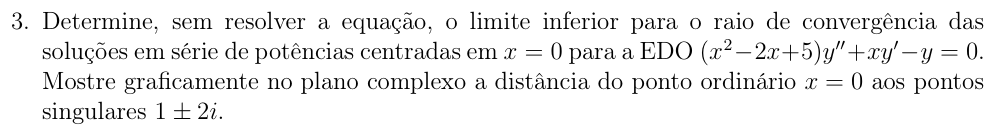
\includegraphics[width=0.8\textwidth]{q3.png}
\end{figure}

\setbeamercolor{block title}{bg=structure.fg, fg=white}
\setbeamercolor{block body}{bg=structure.fg!10, fg=black}

\begin{block}{Conceito chave}
    Para determinar o limite inferior para o raio de convergência da série, devemos verificar a distância do ponto de singularidade complexo mais próximo até o centro da série de expansão.
\end{block}
    
\end{frame}

\begin{frame}{Questão 3 - Resolução (Parte 1)}

    Dada a EDO:
    \[ (x^2 - 2x + 5)y'' + xy' - y = 0 \quad \rightarrow \text{centrada em } x=0 . \]

    Analisando o polinômio que acompanha a derivada de maior ordem para encontrar os pontos singulares:
    \[ x^2 - 2x + 5 = 0 \]
    
    As raízes desse polinômio (pontos singulares) são os números complexos:
    \[ (1+2j) \quad \text{e} \quad (1-2j) \]

\end{frame}

\begin{frame}{Questão 3 - Resolução (Parte 2)}

\begin{minipage}{0.5\textwidth}
\begin{center}
\begin{tikzpicture}
    % Eixos
    \draw[->] (-1,0) -- (3,0) node[right] {$Re$};
    \draw[->] (0,-3) -- (0,3) node[above] {$Im$};

    % Origem e marcações
    \node[below left] at (0,0) {$0$};
    \draw (1,0.1) -- (1,-0.1) node[below] {$1$};
    \draw (0.1,2) -- (-0.1,2) node[left] {$2$};
    \draw (0.1,-2) -- (-0.1,-2) node[left] {$-2$};

    % Pontos singulares
    \filldraw (1,2) circle (1.5pt) node[right] {$P(1+2j)$};
    \filldraw (1,-2) circle (1.5pt) node[right] {$(1-2j)$};

    % Distância r
    \draw (0,0) -- (1,2) node[midway, above left] {$r$};
    \draw (0,0) -- (1,-2) node[midway, below left] {$r$};
    
    % Linhas tracejadas
    \draw[dashed] (1,0) -- (1,2);
    \draw[dashed] (1,0) -- (1,-2);
\end{tikzpicture}
\end{center}
\end{minipage}%
\begin{minipage}{0.5\textwidth}
    A distância da origem ($x=0$) até os pontos singulares no plano complexo é dada pelo módulo:
    \[ d = |1 \pm 2j| = \sqrt{1^2 + 2^2} = \sqrt{5} \]
    
    \vspace{0.5cm}
    \noindent Portanto, o limite inferior do raio de convergência é $\sqrt{5}$.
\end{minipage}

\end{frame}

%=====================================================================================
\subsection{Questão 4}

\begin{frame}{Questão 4 - Enunciado}
\begin{figure}[h]
     \centering
    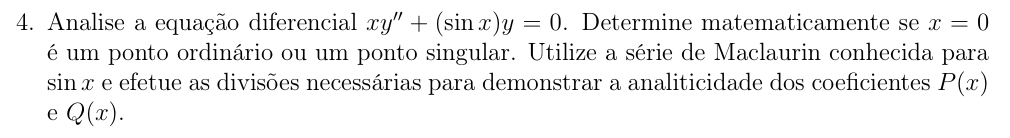
\includegraphics[width=0.8\textwidth]{q4.png}
\end{figure}
\end{frame}

\begin{frame}[allowframebreaks]{Questão 4 - Resolução}
    
    \textbf{1ª Solução (Aproximação para pequenos ângulos):}
    
    \[ xy'' + \text{sen}(x)y = 0 \quad \left(\cdot \frac{1}{x}\right) \]
    \[ y'' + \frac{\text{sen}(x)}{x} y = 0 \]
    
    Para valores de $x$ muito próximos a zero, podemos usar a aproximação $\text{sen}(x) \simeq x$.
    
    Portanto, para $x \to 0$:
    \[ y'' + \frac{x}{x}y = 0 \implies \boxed{y'' + y = 0} \]
    
    \begin{itemize}
        \item Isso indica que a equação se comporta de forma analítica em $x=0$.
    \end{itemize}

    \framebreak 
    
    \textbf{2ª Solução (Expansão em Série de Taylor):}
    
    \[ y'' + \underbrace{\left( \frac{\text{sen}(x)}{x} \right)}_{\text{Expansão de Taylor em } x=0} y = 0 \]
    
    Temos que a expansão em série de Maclaurin para $\text{sen}(x)$ é:
    \[ \text{sen}(x) = \sum_{n=0}^{\infty} \frac{\text{sen}^{(n)}(0)}{n!} x^n = x - \frac{x^3}{3!} + \frac{x^5}{5!} - \dots = \sum_{n=0}^{\infty} \frac{(-1)^n x^{2n+1}}{(2n+1)!} \]
    
    Sendo $P(x) = \frac{\text{sen}(x)}{x}$, substituímos a série:
    \begin{align*}
        P(x) &= \frac{1}{x} \sum_{n=0}^{\infty} \frac{(-1)^n x^{2n+1}}{(2n+1)!} \\[1ex]
        P(x) &= \frac{1}{x} \left( x - \frac{x^3}{3!} + \frac{x^5}{5!} - \frac{x^7}{7!} + \dots \right) \\[1ex]
        P(x) &= 1 - \frac{x^2}{3!} + \frac{x^4}{5!} - \frac{x^6}{7!} + \dots 
    \end{align*}
    
    \framebreak 
    
    \setbeamercolor{block title}{bg=structure.fg, fg=white}
    \setbeamercolor{block body}{bg=structure.fg!10, fg=black}

    \begin{block}{Conclusão}
        Como a expansão resulta em uma série de potências bem definida em $x=0$:
        \[ \therefore P(x) = \sum_{n=0}^{\infty} \frac{(-1)^n x^{2n}}{(2n+1)!} \quad \longrightarrow \quad \text{Converge em todo } x \in \mathbb{R}. \]
        Logo, $x=0$ é um ponto ordinário.
    \end{block}
    
\end{frame}

%=====================================================================================
\subsection{Questão 5}

\begin{frame}{Questão 5 - Enunciado}

\begin{figure}[h]
    \centering
    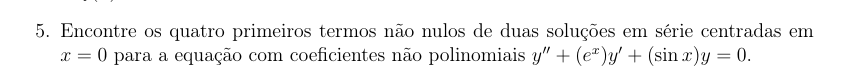
\includegraphics[width=0.8\textwidth]{q5.png}
\end{figure}

\setbeamercolor{block title}{bg=structure.fg, fg=white}
\setbeamercolor{block body}{bg=structure.fg!10, fg=black}
  
  \begin{block}{Conceito chave:}
    É necessária uma análise da série centrada em zero para cada termo da equação diferencial. Para os termos $e^x$ e $\text{sen}(x)$, utilizaremos suas respectivas expansões em série de Maclaurin.
  \end{block}

\end{frame}


\begin{frame}

    Dada a equação diferencial regular em $x=0$:
    \begin{equation*}
        y'' + e^x y' + \text{sen}(x) y = 0
    \end{equation*}

    As séries para as funções e a solução são assumidas como:
    \begin{align*}
        y(x) &= \sum_{n=0}^{\infty} c_n x^n = c_0 + c_1 x + c_2 x^2 + c_3 x^3 + c_4 x^4 + \dots \\
        y'(x) &= \sum_{n=1}^{\infty} c_n n x^{n-1} = c_1 + 2c_2 x + 3c_3 x^2 + 4c_4 x^3 + 5c_5 x^4 + \dots \\
        y''(x) &= \sum_{n=2}^{\infty} c_n n(n-1) x^{n-2} = 2c_2 + 6c_3 x + 12c_4 x^2 + 20c_5 x^3 + \dots
    \end{align*}
    
    Expansões de Taylor conhecidas que serão substituídas na EDO:
    \begin{align*}
        e^x &= \sum_{n=0}^{\infty} \frac{x^n}{n!} = 1 + x + \frac{x^2}{2!} + \frac{x^3}{3!} + \frac{x^4}{4!} + \dots \\
        \text{sen}(x) &= \sum_{n=0}^{\infty} (-1)^n \frac{x^{2n+1}}{(2n+1)!} = x - \frac{x^3}{3!} + \frac{x^5}{5!} - \dots
    \end{align*}
\end{frame}

\begin{frame}{Questão 5 - Identidade de Polinômios (Graus 0 e 1)}
    Substituindo as séries na EDO e agrupando os termos:
    
    \vspace{0.5cm}
    \textbf{Primeiros termos constantes (grau 0):}
    \begin{equation*}
        2c_2 + c_1(1) = 0 \implies 2c_2 = -c_1 \implies c_2 = -\frac{c_1}{2}
    \end{equation*}
    
    \vspace{0.5cm}
    \textbf{Para termos de grau $x^1$:}
    \begin{align*}
        6c_3 x + c_1 x + 2c_2 x + c_0 x &= 0 \\
        6c_3 + c_1 - c_1 + c_0 &= 0 \\
        6c_3 + c_0 &= 0 \implies c_3 = -\frac{c_0}{6}
    \end{align*}
\end{frame}

\begin{frame}{Questão 5 - Identidade de Polinômios (Graus 2 e 3)}
    \textbf{Para termos de grau $x^2$:}
    \begin{align*}
        12c_4 x^2 + 3c_3 x^2 + 2c_2 x^2 + c_1 \frac{x^2}{2} + c_1 x^2 &= 0 \\
        12c_4 - \frac{c_0}{2} - c_1 + \frac{c_1}{2} + c_1 &= 0 \\
        12c_4 - \frac{c_0}{2} + \frac{c_1}{2} &= 0 \implies c_4 = \frac{c_0}{24} - \frac{c_1}{24}
    \end{align*}
    
    \vspace{0.5cm}
    \textbf{Para termos de grau $x^3$:}
    \begin{align*}
        20c_5 x^3 + 4c_4 x^3 + 3c_3 x^3 + 2c_2 \frac{x^3}{2} + c_1 \frac{x^3}{6} + c_2 x^3 - c_0 \frac{x^3}{6} &= 0
    \end{align*}
    Simplificando as constantes, obtemos:
    \begin{equation*}
        20c_5 = \frac{c_0}{2} + c_1 \implies c_5 = \frac{c_0}{40} + \frac{c_1}{20}
    \end{equation*}
\end{frame}

\begin{frame}{Questão 5 - Soluções Fundamentais $y_1(x)$ e $y_2(x)$}
    \textbf{Para $y_1(x)$ (fazendo $c_1 = 0$ e $c_0 = 1$):}
    \begin{itemize}
        \item $c_2 = 0$
        \item $c_3 = -c_0/6$
        \item $c_4 = c_0/24$
        \item $c_5 = c_0/40$
    \end{itemize}
    \begin{equation*}
        y_1(x) = c_0 \left( 1 - \frac{x^3}{6} + \frac{x^4}{24} + \frac{x^5}{40} + \dots \right)
    \end{equation*}
    
    \vspace{0.3cm}
    \textbf{Para $y_2(x)$ (fazendo $c_1 = 1$ e $c_0 = 0$):}
    \begin{itemize}
        \item $c_2 = -c_1/2$
        \item $c_3 = 0$
        \item $c_4 = -c_1/24$
        \item $c_5 = c_1/20$
    \end{itemize}
    \begin{equation*}
        y_2(x) = c_1 \left( x - \frac{x^2}{2} - \frac{x^4}{24} + \frac{x^5}{20} + \dots \right)
    \end{equation*}
\end{frame}

\begin{frame}{Questão 5 - Solução Geral}
    A solução geral é dada pela combinação linear das soluções fundamentais:
    \begin{equation*}
        y(x) = y_1(x) + y_2(x)
    \end{equation*}
    
    Portanto, substituindo as expansões dos termos encontrados, temos a solução em série truncada até $x^5$:
    \begin{equation*}
        y(x) = c_0 \left( 1 - \frac{x^3}{6} + \frac{x^4}{24} + \frac{x^5}{40} \right) + c_1 \left( x - \frac{x^2}{2} - \frac{x^4}{24} + \frac{x^5}{20} \right)
    \end{equation*}
\end{frame}

%=====================================================================================
\subsection{Questão 6}

\begin{frame}{Questão 6 - Enunciado}

\begin{figure}[h]
    \centering
    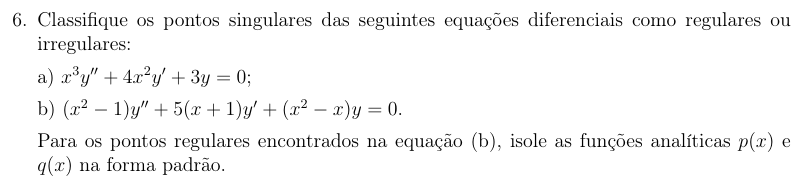
\includegraphics[width=0.8\textwidth]{q6.png}
\end{figure}

\end{frame}

\begin{frame}{Questão 6 - Resolução Letra a)}
    \textbf{a)} Dada a equação diferencial:
    \begin{equation*}
        x^3 y'' + 4x^2 y' + 3y = 0
    \end{equation*}

    Dividindo toda a equação pela maior potência ($x^3$), obtemos a forma padrão:
    \begin{equation*}
        \therefore y'' + \frac{4}{x} y' + \frac{3}{x^3} y = 0
    \end{equation*}

    Temos o ponto singular em:
    \begin{equation*}
        x = 0
    \end{equation*}

    \vspace{0.5cm}
    $\hookrightarrow$ Devido a $x=0$ ser um ponto singular cujos termos $x P(x)$ ou $x^2 Q(x)$ não são analíticos, teremos um \textbf{ponto singular irregular}.
\end{frame}

\begin{frame}
    \textbf{b)} Dada a equação diferencial:
    \begin{equation*}
        (x^2-1)y'' + 5(x+1)y' + (x^2-x)y = 0
    \end{equation*}

    Colocando na forma padrão (dividindo por $x^2-1$) e fatorando os polinômios:
    \begin{equation*}
        y'' + \frac{5(x+1)}{(x+1)(x-1)} y' + \frac{x\cancel{(x-1)}}{(x+1)\cancel{(x-1)}} y = 0
    \end{equation*}

    Simplificando a expressão, obtemos as funções $P(x)$ e $Q(x)$:
    \begin{align*}
        P(x) &= \frac{5}{x-1} \\[10pt]
        Q(x) &= \frac{x}{x+1}
    \end{align*}
    
    A equação fica:
    \begin{equation*}
        y'' + \frac{5}{x-1} y' + \frac{x}{x+1} y = 0
    \end{equation*}

    \vspace{0.3cm}
  

  
    $\hookrightarrow$ Avaliando os limites, concluímos que temos um \textbf{ponto singular regular}.
\end{frame}
      
%=====================================================================================
\subsection{Questão 7}

\begin{frame}{Questão 7 - Enunciado}

\begin{figure}[h]
    \centering
    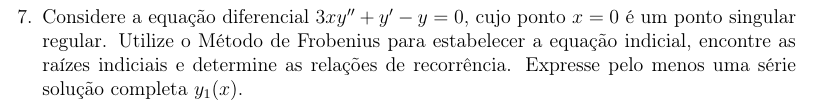
\includegraphics[width=0.8\textwidth]{q7.png}
\end{figure}

\setbeamercolor{block title}{bg=structure.fg, fg=white}
\setbeamercolor{block body}{bg=structure.fg!10, fg=black}
  
  \begin{block}{Conceito chave:}
   Devido a equação apresentar um ponto singular em $x=0$, assumimos a hipótese de solução conforme a definição do Método de Frobenius:
\[
y(x) = x^{r} \sum_{n=0}^{\infty} c_{n} x^{n}
\]
  \end{block}

\end{frame}

\begin{frame}{Questão 7 - Análise do Ponto Singular}
    Dada a equação diferencial:
    \begin{equation*}
        3xy'' + y' - y = 0 \quad ; \quad \exists \text{ um ponto singular em } x=0
    \end{equation*}
    Pois, ao dividir por $3x$:
    \begin{equation*}
        y'' + \frac{y'}{3x} - \frac{y}{3x} = 0 \quad ; \quad \nexists \text{ solução analítica } \in \mathbb{R} \text{ para } x=0
    \end{equation*}
    
    Portanto, assumimos a solução na forma de Frobenius:
    \begin{equation*}
        y(x) = x^r \sum_{n=0}^{\infty} c_n x^n = x^r (c_0 + c_1 x + c_2 x^2 + \dots + c_n x^n)
    \end{equation*}
    Derivando termo a termo:
    \begin{align*}
        y'(x) &= \sum_{n=0}^{\infty} c_n (n+r) x^{n+r-1} \\
        y''(x) &= \sum_{n=0}^{\infty} c_n (n+r)(n+r-1) x^{n+r-2}
    \end{align*}
\end{frame}

\begin{frame}{Questão 7 - Substituição na Equação Diferencial}
    Substituindo na EDO original $3xy'' + y' - y = 0$:
    \begin{multline*}
        3x \sum_{n=0}^{\infty} c_n(n+r)(n+r-1)x^{n+r-2} \\ 
        + \sum_{n=0}^{\infty} c_n(n+r)x^{n+r-1} - \sum_{n=0}^{\infty} c_n x^{n+r} = 0 
    \end{multline*}
    
    Dividindo toda a expressão por $x^r$:
    \begin{equation*}
        \therefore 3 \sum_{n=0}^{\infty} c_n(n+r)(n+r-1)x^{n-1} + \sum_{n=0}^{\infty} c_n(n+r)x^{n-1} - \sum_{n=0}^{\infty} c_n x^n = 0
    \end{equation*}
\end{frame}

\begin{frame}{Questão 7 - Equação Indicial}
    Extraindo o primeiro termo das séries com $x^{n-1}$ (para $n=0$):
    \begin{equation*}
        3\left[c_0(r)(r-1)x^{-1} \right] + \left[c_0(r)x^{-1} \right] + \dots = 0
    \end{equation*}
    
    Analisando os coeficientes da menor potência da variável ($x^{-1}$):
    \begin{align*}
        &3 c_0(r)(r-1) + (r)c_0 = 0 \\
        \therefore \quad &3(r)(r-1) + r = 0 \implies 3r^2 - 3r + r = 0 \\
        &3r^2 - 2r = 0 \implies r(3r - 2) = 0
    \end{align*}
    
    Temos as raízes indiciais:
    \begin{equation*}
        r = 0 \quad \text{ou} \quad r = 2/3
    \end{equation*}
\end{frame}

\begin{frame}{Questão 7 - Ajuste dos Índices da Série}
    Retornando à equação das séries gerais agrupadas:
    \begin{equation*}
        3 \sum_{n=1}^{\infty} c_n(n+r)(n+r-1)x^{n-1} + \sum_{n=1}^{\infty} c_n(n+r)x^{n-1} - \sum_{n=0}^{\infty} c_n x^n = 0
    \end{equation*}
    
    Fazendo a substituição $k = n-1$ nas duas primeiras somas, e usando $k=n$ na terceira:
    \begin{equation*}
        3 \sum_{k=0}^{\infty} c_{k+1}(k+1+r)(k+r)x^k + \sum_{k=0}^{\infty} c_{k+1}(k+1+r)x^k - \sum_{k=0}^{\infty} c_k x^k = 0
    \end{equation*}
\end{frame}

\begin{frame}{Questão 7 - Relação de Recorrência}
    Fatorando o termo $x^k$ das somas para $k \ge 0$:
    \begin{equation*}
        \sum_{k=0}^{\infty} x^k \left[ c_{k+1} \left[ 3(k+1+r)(k+r) + (k+1+r) \right] - c_k \right] = 0
    \end{equation*}
    
    Para que os coeficientes sejam nulos, obtemos a relação de recorrência geral:
    \begin{equation*}
        c_{k+1} = \frac{c_k}{3(k+1+r)(k+r) + (k+1+r)}
    \end{equation*}
\end{frame}

\begin{frame}
    Para a raiz $r=0$, a relação de recorrência simplifica-se para:
    \begin{equation*}
        c_{k+1} = \frac{c_k}{3(k+1)(k) + (k+1)}
    \end{equation*}
    
    \vspace{0.3cm}
    Para \fbox{$k=0$}: 
    \begin{equation*}
        c_1 = \frac{c_0}{3(1)(0) + 1} = c_0
    \end{equation*}
    
    Para \fbox{$k=1$}: 
    \begin{equation*}
        c_2 = \frac{c_1}{3(2)(1) + 2} = \frac{c_1}{8}
    \end{equation*}
    
    Para \fbox{$k=2$}: 
    \begin{equation*}
        c_3 = \frac{c_2}{3(3)(2) + 3} = \frac{c_1/8}{21} = \frac{c_1}{168}
    \end{equation*}
    
    Para \fbox{$k=3$}: 
    \begin{equation*}
        c_4 = \frac{c_3}{3(4)(3) + 4} = \frac{c_1/168}{40} = \frac{c_1}{6720}
    \end{equation*}
\end{frame}

\begin{frame}{Questão 7 - Solução Fundamental $y_1(x)$}
    Com base no formato assumido inicialmente para $r=0$:
    \begin{equation*}
        y_1(x) = x^0 \sum_{n=0}^{\infty} c_n x^n = c_0 + c_1 x + c_2 x^2 + c_3 x^3 + \dots
    \end{equation*}
    
    Considerando a relação de que os termos dependem de $c_1$ a partir de $k=1$, e omitindo o $c_0$ na escrita parcial (fazendo $c_0=0$ na formulação alternativa apresentada nas notas originais, restando $c_1$ em evidência):
    \begin{equation*}
        y_1(x) = c_1 x + \frac{c_1}{8} x^2 + \frac{c_1}{168} x^3 + \frac{c_1}{6720} x^4 + \dots
    \end{equation*}
\end{frame}
  
%=====================================================================================
\subsection{Questão 8}

\begin{frame}{Questão 8 - Enunciado}

\begin{figure}[h]
    \centering
    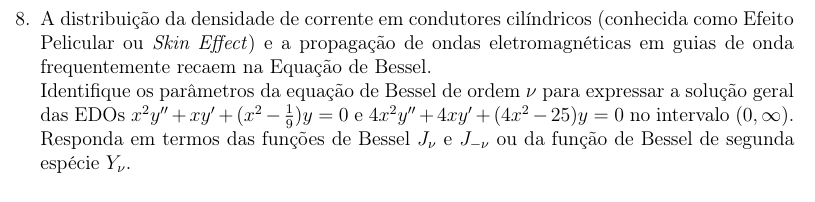
\includegraphics[width=0.8\textwidth]{q8.png}
\end{figure}

\end{frame}

\begin{frame}{Questão 8 - Resolução Letra a)}
    \textbf{a)} Dada a equação diferencial:
    \begin{equation*}
        x^2 y'' + x y' + \left(x^2 - \frac{1}{9}\right)y = 0 
    \end{equation*}
    
    Essa é a Equação de Bessel de ordem $v$, onde:
    \begin{equation*}
        \begin{cases} 
            v^2 = \left(\frac{1}{3}\right)^2 \\ 
            v = 1/3 
        \end{cases}
    \end{equation*}
    
    Como $v = 1/3$ não é um inteiro, a solução geral será uma combinação linear das funções de Bessel de primeira espécie $J_v$ e $J_{-v}$.
    
    \begin{equation*}
        \therefore y(x) = C_1 J_{1/3}(x) + C_2 J_{-1/3}(x)
    \end{equation*}
\end{frame}

\begin{frame}{Questão 8 - Definição das Séries para Letra a)}
    Onde as funções $J_{1/3}$ e $J_{-1/3}$ podem ser definidas por suas expansões em série:
    
    \vspace{0.5cm}
    \begin{equation*}
        J_{1/3}(x) = x^{1/3} \sum_{k=0}^{\infty} \frac{(-1)^k x^{2k}}{2^{2k+1/3} \cdot k! \, \Gamma(4/3+k)}
    \end{equation*}
    
    \vspace{0.5cm}
    \begin{equation*}
        J_{-1/3}(x) = x^{-1/3} \sum_{k=0}^{\infty} \frac{(-1)^k x^{2k}}{2^{2k-1/3} \cdot k! \, \Gamma(2/3+k)}
    \end{equation*}
\end{frame}

\begin{frame}{Questão 8 - Resolução Letra b)}
    \textbf{b)} Dada a equação diferencial:
    \begin{equation*}
        4x^2 y'' + 4xy' + (4x^2 - 25)y = 0 
    \end{equation*}
    
    Deixando no formato padrão da função de Bessel (dividindo tudo por 4):
    \begin{equation*}
        x^2 y'' + x y' + \left(x^2 - \frac{25}{4}\right)y = 0
    \end{equation*}
    
    Identificamos a ordem $v$:
    \begin{equation*}
        v^2 = \frac{25}{4} \implies v = \sqrt{\frac{25}{4}} = \frac{5}{2}
    \end{equation*}
    
    Portanto $v \notin \mathbb{Z}$ e $v \geq 0$.
\end{frame}

\begin{frame}{Questão 8 - Solução Letra b)}
    Logo, de forma semelhante ao item anterior, a solução pode ser definida por uma combinação linear das funções de Bessel de primeira espécie $J_v$ e $J_{-v}$.
    
    Portanto:
    \begin{equation*}
        y(x) = C_1 J_{5/2}(x) + C_2 J_{-5/2}(x)
    \end{equation*}
    
    \vspace{1cm}
    \begin{center}
        \fbox{Podemos deixar também na forma das definições em Séries de Potência.}
    \end{center}
\end{frame}

%=====================================================================================
\subsection{Questão 9}

\begin{frame}{Questão 9 - Enunciado}

\begin{figure}[h]
    \centering
    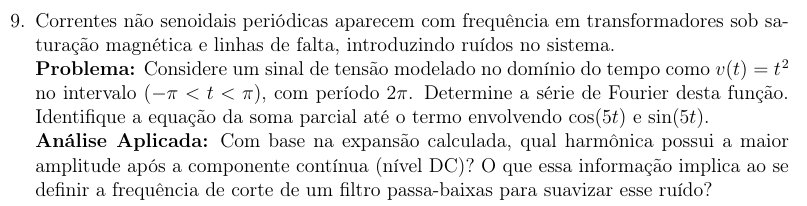
\includegraphics[width=0.8\textwidth]{q9.png}
\end{figure}

\end{frame}

\begin{frame}{Questão 9 - Definição do Problema}
    Dada a função e o intervalo:
    \begin{equation*}
        v(t) = t^2 \quad , \quad t \in (-\pi, \pi) \quad \leftrightarrow \quad (-p, p) \implies p = \pi
    \end{equation*}
    
    Determine a série de Fourier para essa função. A fórmula geral é:
    \begin{equation*}
        v(t) = \frac{a_0}{2} + \sum_{n=1}^{\infty} \left[ a_n \cos\left(\frac{n\pi}{p} t\right) + b_n \text{sen}\left(\frac{n\pi}{p} t\right) \right]
    \end{equation*}
    
    Onde $a_0$ representa a componente DC do sistema, $a_n$ os coeficientes dos termos pares (cossenos) e $b_n$ os termos ímpares (senos).
\end{frame}

\begin{frame}{Questão 9 - Componente DC ($a_0$)}
    Calculando o coeficiente $a_0$:
    \begin{equation*}
        a_0 = \frac{1}{p} \int_{-p}^{p} v(t) dt = \frac{1}{\pi} \int_{-\pi}^{\pi} t^2 dt
    \end{equation*}
    
    Resolvendo a integral analiticamente:
    \begin{align*}
        a_0 &= \frac{1}{\pi} \left[ \frac{t^3}{3} \right]_{-\pi}^{\pi} = \frac{1}{\pi} \left( \frac{\pi^3}{3} - \frac{(-\pi)^3}{3} \right) = \frac{1}{\pi} \left( \frac{\pi^3}{3} + \frac{\pi^3}{3} \right) \\[10pt]
        a_0 &= \frac{2\pi^2}{3} \cong 6,5797
    \end{align*}
\end{frame}

\begin{frame}{Questão 9 - Componente Par ($a_n$) - Parte 1}
    Calculando os coeficientes $a_n$:
    \begin{equation*}
        a_n = \frac{1}{p} \int_{-p}^{p} v(t) \cos\left(\frac{n\pi t}{p}\right) dt = \frac{1}{\pi} \int_{-\pi}^{\pi} t^2 \cos(nt) dt 
    \end{equation*}
    
    Para resolver a integral, utilizaremos o método de integração por partes (LIATE):
    \begin{align*}
        u &= t^2 \implies du = 2t \, dt \\
        dV &= \cos(nt) \, dt \implies v = \int \cos(nt) dt = \frac{1}{n} \text{sen}(nt)
    \end{align*}
    
    \begin{equation*}
        \therefore \int t^2 \cos(nt) dt = t^2 \frac{1}{n} \text{sen}(nt) - \frac{2}{n} \int t \text{sen}(nt) \, dt
    \end{equation*}
\end{frame}

\begin{frame}{Questão 9 - Componente Par ($a_n$) - Parte 2}
    Integrando por partes novamente o segundo termo $\int t \text{sen}(nt) \, dt$:
    \begin{equation*}
        \int t^2 \cos(nt) dt = \frac{t^2}{n} \text{sen}(nt) - \frac{2}{n} \left[ -\frac{t}{n} \cos(nt) + \frac{1}{n^2} \text{sen}(nt) \right]
    \end{equation*}
    
    Aplicando os limites de integração no intervalo de $-\pi$ a $\pi$:
    \begin{equation*}
        a_n = \frac{1}{\pi} \left[ \frac{1}{n} \text{sen}(nt) \left( t^2 - \frac{2}{n^2} \right) + \frac{2t}{n^2} \cos(nt) \right]_{-\pi}^{\pi}
    \end{equation*}
    
    Como $\text{sen}(\pm n\pi) = 0$ e $\cos(\pm n\pi) = (-1)^n$:
    \begin{equation*}
        a_n = \frac{1}{\pi} \left( \frac{2\pi}{n^2} \cos(n\pi) - \left(-\frac{2\pi}{n^2} \cos(-n\pi)\right) \right) = \frac{4}{n^2} (-1)^n
    \end{equation*}
\end{frame}

\begin{frame}{Questão 9 - Componente Ímpar ($b_n$) - Parte 1}
    Calculando os coeficientes $b_n$:
    \begin{equation*}
        b_n = \frac{1}{p} \int_{-p}^{p} v(t) \text{sen}\left(\frac{n\pi t}{p}\right) dt = \frac{1}{\pi} \int_{-\pi}^{\pi} t^2 \text{sen}(nt) dt
    \end{equation*}
    
    Aplicando integração por partes:
    \begin{align*}
        u &= t^2 \implies du = 2t \, dt \\
        dV &= \text{sen}(nt) \, dt \implies v = -\frac{1}{n} \cos(nt)
    \end{align*}
    
    \begin{equation*}
        \therefore \int t^2 \text{sen}(nt) dt = -\frac{1}{n} t^2 \cos(nt) + \frac{2}{n} \int t \cos(nt) \, dt
    \end{equation*}
\end{frame}

\begin{frame}{Questão 9 - Componente Ímpar ($b_n$) - Parte 2}
    Integrando o termo final:
    \begin{equation*}
        \therefore \int t^2 \text{sen}(nt) dt = -\frac{t^2}{n} \cos(nt) + \frac{2}{n} \left[ \frac{t}{n} \text{sen}(nt) + \frac{\cos(nt)}{n^2} \right]
    \end{equation*}
    
    Agrupando os terms:
    \begin{equation*}
        \int t^2 \text{sen}(nt) dt = \frac{\cos(nt)}{n} \left[ \frac{2}{n^2} - t^2 \right] + \frac{2t}{n^2} \text{sen}(nt)
    \end{equation*}
    
    Aplicando os limites simétricos de $-\pi$ a $\pi$ em uma função ímpar original ($t^2 \text{sen}(nt)$):
    \begin{align*}
        b_n &= \frac{1}{\pi} \left[ \frac{\cos(nt)}{n} \left( \frac{2}{n^2} - t^2 \right) + \frac{2t}{n^2} \text{sen}(nt) \right]_{-\pi}^{\pi} \\[10pt]
        b_n &= \frac{1}{\pi} ( 0 ) = 0 \quad ; \quad \forall n \in \mathbb{Z}
    \end{align*}
\end{frame}

\begin{frame}{Questão 9 - Definição da Série de Fourier Final}
    Substituindo os coeficientes encontrados, a Série de Fourier é:
    \begin{equation*}
        V(t) = \frac{a_0}{2} + \sum_{n=1}^{\infty} a_n \cos(nt) = \frac{\pi^2}{3} + \sum_{n=1}^{\infty} \frac{4(-1)^n}{n^2} \cos(nt)
    \end{equation*}
    
    Expandindo até o termo $\cos(5t)$, teremos:
    \begin{multline*}
        V(t) = \frac{\pi^2}{3} + \left[ -4 \cos(t) + \frac{4}{4} \cos(2t) - \frac{4}{9} \cos(3t) \right. \\
        \left. + \frac{4}{16} \cos(4t) - \frac{4}{25} \cos(5t) \right]
    \end{multline*}
    
    \begin{equation*}
        \therefore V(t) = \frac{\pi^2}{3} - 4 \cos(t) + \cos(2t) - \frac{4}{9} \cos(3t) + \frac{1}{4} \cos(4t) - \frac{4}{25} \cos(5t) + \dots
    \end{equation*}
    
    \vspace{0.3cm}
    Analisando o termo $\frac{4(-1)^n}{n^2}$, vemos que para $n=1$ teremos a harmônica com a maior amplitude em módulo.
\end{frame}

%=====================================================================================
\subsection{Questão 10}

\begin{frame}{Questão 10 - Enunciado}

\begin{figure}[h]
    \centering
    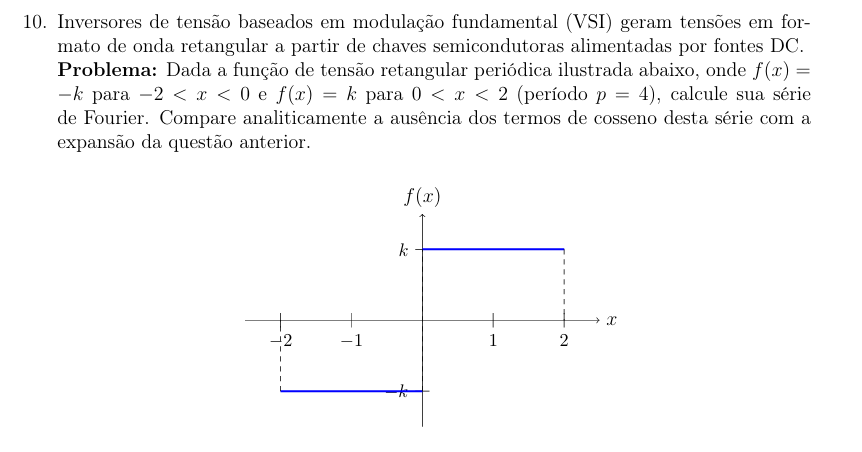
\includegraphics[width=0.8\textwidth]{q10.png}
\end{figure}

\end{frame}

\begin{frame}{Questão 10 - Definição da Função}
    Dada a função por partes no intervalo $[-P, P] = [-2, 2]$:
    \begin{equation*}
        f(x) = \begin{cases} 
            -k & \text{, se } -2 < x < 0 \\ 
            +k & \text{, se } 0 < x < 2 
        \end{cases}
    \end{equation*}
    
    A representação em série de Fourier é dada por:
    \begin{equation*}
        f(x) = \frac{a_0}{2} + \sum_{n=1}^{\infty} \left[ a_n \cos\left(\frac{n\pi x}{2}\right) + b_n \text{sen}\left(\frac{n\pi x}{2}\right) \right]
    \end{equation*}
\end{frame}

\begin{frame}{Questão 10 - Componente DC ($a_0$)}
    Calculando a componente DC:
    \begin{equation*}
        a_0 = \frac{1}{p} \int_{-p}^{p} f(x) dx = \frac{1}{2} \int_{-2}^{2} f(x) dx = \frac{1}{2} \left[ \int_{-2}^{0} -k \, dx + \int_{0}^{2} k \, dx \right]
    \end{equation*}
    
    Resolvendo as integrais:
    \begin{align*}
        a_0 &= \frac{1}{2} \left[ -kx \Big|_{-2}^{0} + kx \Big|_{0}^{2} \right] = \frac{1}{2} \left[ (-k(0) - (-k(-2))) + (k(2) - k(0)) \right] \\[10pt]
        a_0 &= \frac{1}{2} \left[ -2k + 2k \right] = 0
    \end{align*}
    
    \vspace{0.5cm}
    Componente DC numericamente igual a zero (função possui simetria).
\end{frame}

\begin{frame}{Questão 10 - Componente Par ($a_n$)}
    Calculando a componente par:
    \begin{equation*}
        a_n = \frac{1}{p} \int_{-p}^{p} f(x) \cos\left(\frac{n\pi x}{p}\right) dx = \frac{1}{2} \int_{-2}^{2} f(x) \cos\left(\frac{n\pi x}{2}\right) dx
    \end{equation*}
    
    Dividindo nos subintervalos:
    \begin{equation*}
        a_n = \frac{1}{2} \left[ \int_{-2}^{0} -k \cos\left(\frac{n\pi x}{2}\right) dx + \int_{0}^{2} k \cos\left(\frac{n\pi x}{2}\right) dx \right]
    \end{equation*}
    
    Integrando:
    \begin{equation*}
        a_n = \frac{1}{2} \left[ \left( -\frac{2k}{n\pi} \text{sen}\left(\frac{n\pi x}{2}\right) \right) \Bigg|_{-2}^{0} + \left( \frac{2k}{n\pi} \text{sen}\left(\frac{n\pi x}{2}\right) \right) \Bigg|_{0}^{2} \right]
    \end{equation*}
    
    \begin{equation*}
        a_n = \frac{1}{2} [ 0 + 0 ] = 0
    \end{equation*}
    
    \vspace{0.3cm}
    Componente par igual a zero, pois $\text{sen}(\pm n\pi) = 0$ para $n \in \mathbb{Z}$.
\end{frame}

\begin{frame}{Questão 10 - Componente Ímpar ($b_n$) - Parte 1}
    Calculando a componente ímpar:
    \begin{equation*}
        b_n = \frac{1}{p} \int_{-p}^{p} f(x) \text{sen}\left(\frac{n\pi x}{p}\right) dx = \frac{1}{2} \int_{-2}^{2} f(x) \text{sen}\left(\frac{n\pi x}{2}\right) dx
    \end{equation*}
    
    Portanto:
    \begin{equation*}
        b_n = \frac{1}{2} \left[ \int_{-2}^{0} -k \text{sen}\left(\frac{n\pi x}{2}\right) dx + \int_{0}^{2} k \text{sen}\left(\frac{n\pi x}{2}\right) dx \right]
    \end{equation*}
    
    Integrando:
    \begin{equation*}
        \therefore b_n = \frac{1}{2} \left[ \left( \frac{2k}{n\pi} \cos\left(\frac{n\pi x}{2}\right) \right) \Bigg|_{-2}^{0} + \left( -\frac{2k}{n\pi} \cos\left(\frac{n\pi x}{2}\right) \right) \Bigg|_{0}^{2} \right]
    \end{equation*}
\end{frame}

\begin{frame}{Questão 10 - Componente Ímpar ($b_n$) - Parte 2}
    Aplicando os limites de integração e lembrando que $\cos(0)=1$ e $\cos(\pm n\pi) = (-1)^n$:
    \begin{equation*}
        b_n = \frac{1}{2} \left[ \left( \frac{2k}{n\pi} - \frac{2k(-1)^n}{n\pi} \right) + \left( -\frac{2k(-1)^n}{n\pi} + \frac{2k}{n\pi} \right) \right]
    \end{equation*}
    
    Agrupando os termos semelhantes:
    \begin{align*}
        b_n &= \frac{1}{2} \left[ \frac{4k}{n\pi} - \frac{4k(-1)^n}{n\pi} \right] = \frac{2k}{n\pi} - \frac{2k(-1)^n}{n\pi} \\[10pt]
        &= \frac{2k}{n\pi} \left[ 1 - (-1)^n \right]
    \end{align*}
\end{frame}

\begin{frame}{Questão 10 - Série de Fourier Final}
    Como a função $f(x)$ é ímpar, os coeficientes $a_0 = 0$ e $a_n = 0$. A série é composta apenas pelos termos em seno:
    \begin{equation*}
        f(x) = \sum_{n=1}^{\infty} b_n \text{sen}\left(\frac{n\pi x}{2}\right)
    \end{equation*}
    
    Substituindo o valor encontrado para $b_n$, chegamos à expressão final:
    \begin{equation*}
        \therefore f(x) = \sum_{n=1}^{\infty} \left[ \frac{2k}{n\pi} (1 - (-1)^n) \right] \text{sen}\left(\frac{n\pi x}{2}\right)
    \end{equation*}
\end{frame}
  
\section{Conclusão}

\begin{frame}{Conclusão}
    Neste trabalho, apresentamos as resoluções detalhadas de 10 questões, abrangendo equações diferenciais ordinárias (EDOs) e ferramentas associadas: 
    \begin{itemize}
        \item Soluções em séries de potências para pontos ordinários.
        \item Análise de raios e intervalos de convergência.
        \item Classificação de pontos singulares regulares e irregulares.
        \item Aplicação do método de Frobenius.
        \item Expansões e aproximações em Séries de Fourier para funções contínuas e descontínuas (definidas por partes).
    \end{itemize}
    \vspace{0.5cm}
    \centering \textbf{Fim da apresentação.}
\end{frame}

\end{document}